% documentclass
% set font size=11 (11pt)
% set paper format=A4 (a4paper)
% set equation alignment to left (fleqn)
\documentclass[11pt,a4paper,fleqn]{article}


% Preamble
% use the inputenc and fontenc packages to use French accents
\usepackage[utf8]{inputenc}
\usepackage[T1]{fontenc}
% for matrices / vectors
\usepackage{amsmath}
% for references
\usepackage{hyperref}
% allow for arbitrary font size
\usepackage{anyfontsize}
% for color
\usepackage{xcolor}
% for pseudocolor
\usepackage{algorithm,algpseudocode}
% for code samples
\usepackage{listings}
% set the font as Time New Roman (the Latex equivalent, at least)
% \usepackage{mathptmx}
% set the size of the document margins using the geometry package
\usepackage[lmargin=0.97in,rmargin=0.97in,tmargin=1.4in,bmargin=1.4in]{geometry}
% turn the color of footnote markers to black
\renewcommand\thefootnote{\textcolor{black}{\arabic{footnote}}}
% suppress indents on footnotes
\usepackage[hang,flushmargin]{footmisc}
% automatically generates colored brackets around references
\usepackage{fncylab} \labelformat{equation}{(#1)}
% supress indent on new paragraphs
\setlength{\parindent}{0pt}
% use the amsmath package to include mathematical symbols
\usepackage{amsmath}
% suppress the space between the left margin and the equations (fleqn still leaves some space by default)
\setlength{\mathindent}{0pt}
% create a new environment to left flush the equation with the align environment
\makeatletter
\newenvironment{lflalign}{ \vspace{-3mm}%
  \def\align@preamble{%
    &\strut@
    \setboxz@h{\@lign$\m@th\displaystyle{####}$}%
    \ifmeasuring@\savefieldlength@\fi
    \set@field
    \hfil
    \tabskip\z@skip
    &\setboxz@h{\@lign$\m@th\displaystyle{{}####}$}%
    \ifmeasuring@\savefieldlength@\fi
    \set@field
    \hfil
    \tabskip\alignsep@
  }
  \flalign}
{\endflalign}
\makeatother
% use the ammssymb package to use mathematical symbols
\usepackage{amssymb}
% create new commands for mathematical symbols
\DeclareMathOperator{\N}{\mathbb{N}}
\DeclareMathOperator{\Z}{\mathbb{Z}}
\DeclareMathOperator{\Q}{\mathbb{Q}}
\DeclareMathOperator{\R}{\mathbb{R}}
\DeclareMathOperator{\Pb}{\mathbb{P}}
% declare the cmsy (computer modern symbol) math alphabet to define appropriate fonts for the U and N mathematical symbols
\DeclareMathAlphabet\mathbcal{OMS}{cmsy}{m}{n}
% create new commands for mathematical symbols
\DeclareMathOperator{\E}{\mathbcal{E}}
\DeclareMathOperator{\Ex}{\mathbb{E}}
\DeclareMathOperator{\F}{\mathbcal{F}}
\DeclareMathOperator{\G}{\mathbcal{G}}
\DeclareMathOperator{\M}{\mathbcal{M}}
\DeclareMathOperator{\HH}{\mathbcal{H}}
\DeclareMathOperator{\QQ}{\mathbcal{Q}}
\DeclareMathOperator{\PP}{\mathbcal{P}}
\DeclareMathOperator{\Noo}{\mathbcal{N}}
\DeclareMathOperator{\U}{\mathbcal{U}}
% use the bbm package to be able to use the double stroke 1 for the indicator function
\usepackage{bbm}
\DeclareMathOperator{\ind}{\mathbbmss{1}}
% use the bm package to use bold characters in math mode
\usepackage{bm}
% create a new command for black square bullets
\newcommand{\bs}{\scalebox{0.7}{$\blacksquare$} \hspace{2mm}}
% use the relsize package to be abe to change the size of mathematical symbols
\usepackage{relsize}
% define a new command for in-line small summation
\newcommand{\ssumm}[2]{\underset{\scriptscriptstyle #1}{\overset{\scriptscriptstyle #2}{\mathlarger{\mathlarger{\mathlarger{\Sigma}}}}} \hspace{0.5mm}}
% define a new command for in-line small products
\newcommand{\sprod}[2]{\underset{\scriptscriptstyle #1}{\overset{\scriptscriptstyle #2}{\mathlarger{\mathlarger{\mathlarger{\Pi}}}}} \hspace{0.5mm}}
% Use the caption package to customize captions (titles) of tables and graphs
\usepackage[font=small,labelfont=bf]{caption}
% use float package to force figure the be positioned where indicated
\usepackage{float}
% use the graphicx package to be able to resize tables
\usepackage{graphicx}


\begin{document}

% command to check unused bibliography entries
% \nocite{*}

{\fontsize{20pt}{22pt}\selectfont \textbf{How to build a neural network playground from scratch} \par}
\begin{center}
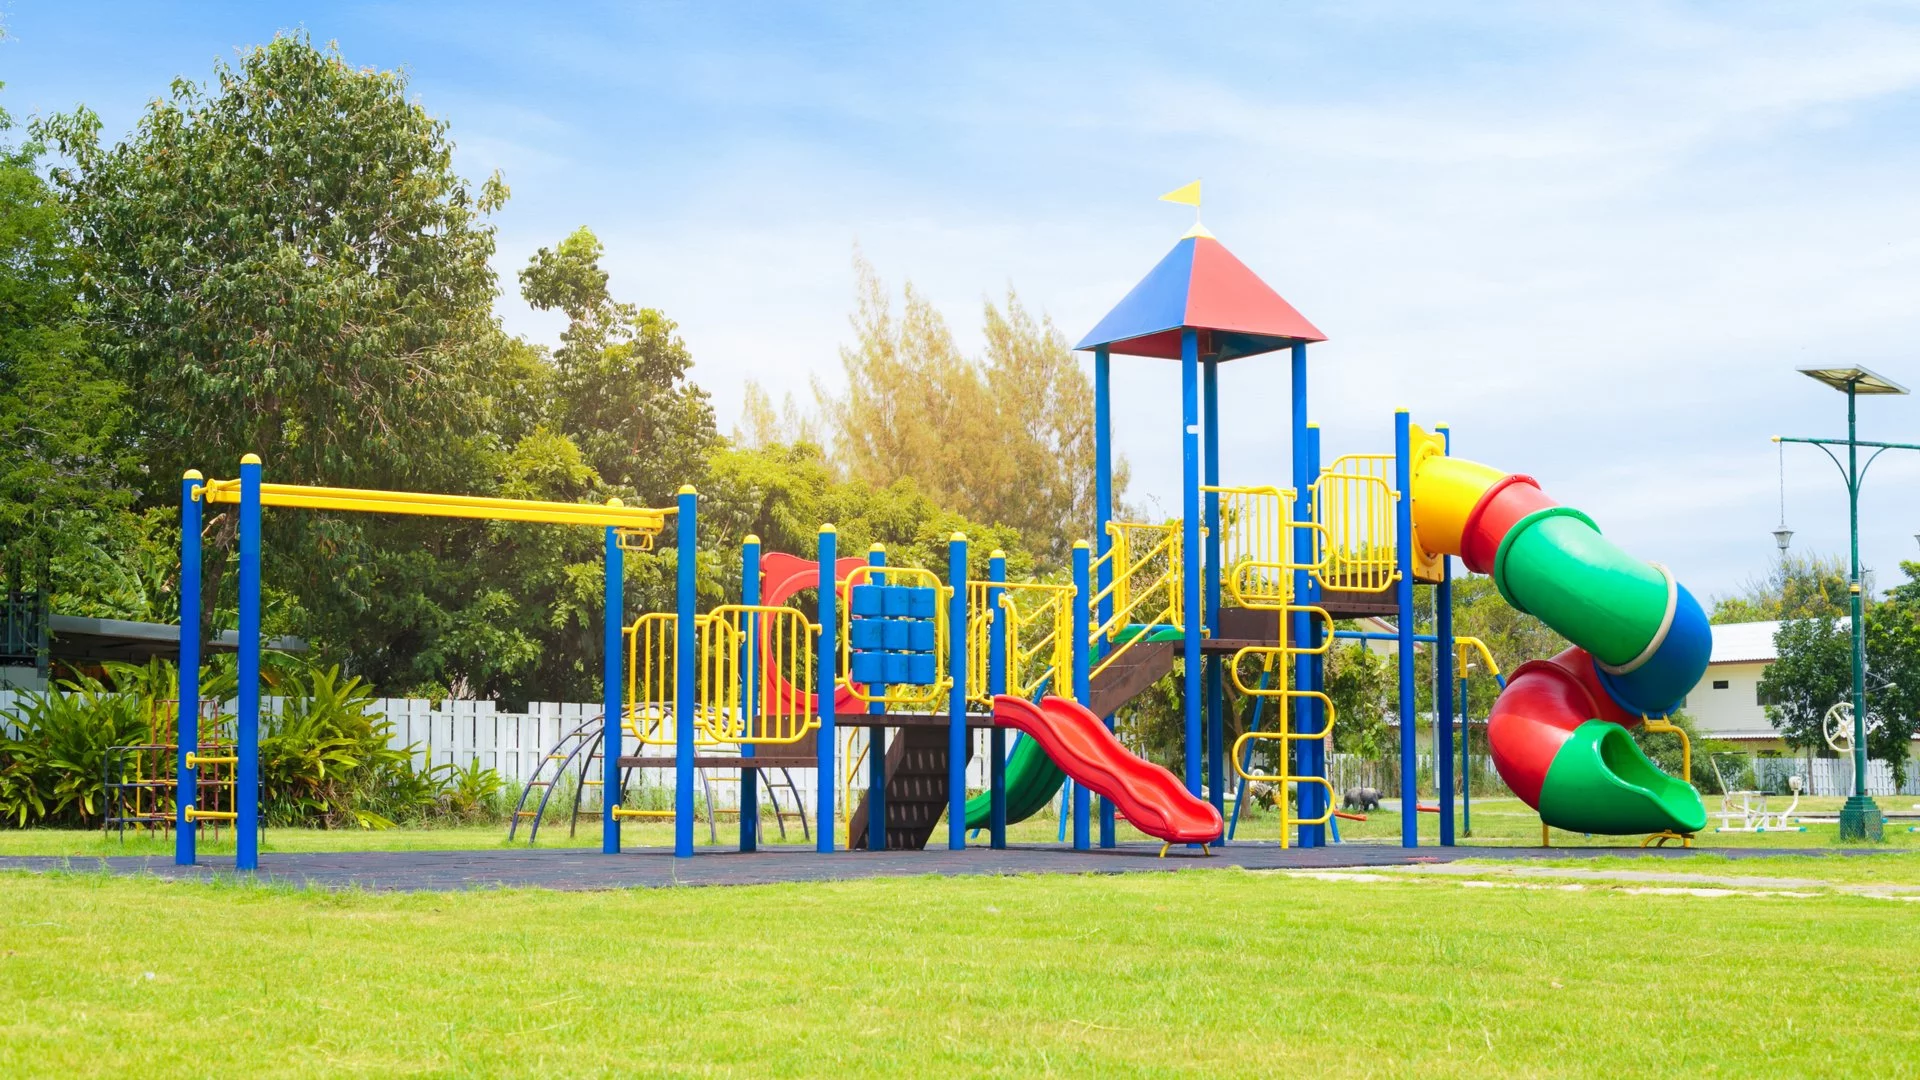
\includegraphics[scale=0.25]{img/playground.png}
\end{center}

\section{Intro}

Neural networks became increasingly popular as shown by the \href{https://www.kdnuggets.com/wp-content/uploads/Fig2-winning-machine-learning-competition.jpg}{research publication topics} of the recent years. The main advantage of those models is that they can learn complex structures and are highly customizable. However, one significant drawback is their poor explanability power. Neural networks are often categorized in the so-called "black box models" that are hard to understand.
Fortunately, there are some very good tutorials to understand how a neural network actually works. The tutorials of \href{https://www.coursera.org/learn/neural-networks-deep-learning}{Andrew Ng} is an example of some very good materials available online. \\

I personally find that a 1-layer network is relatively easy to understand, however it gets tricky when increasing the number of layers. This article is an attempt to understand in details the 2-layer neural network through the building of a small playground. We will even publish the playground \href{https://nn-playground-app.herokuapp.com/}{online}! To enjoy fully this article, the reader must be familiar with the working of a 1-layer neural network.\\

The difference between a 1-layer network and a 2-layer network relies in the following picture: \\

\begin{center}
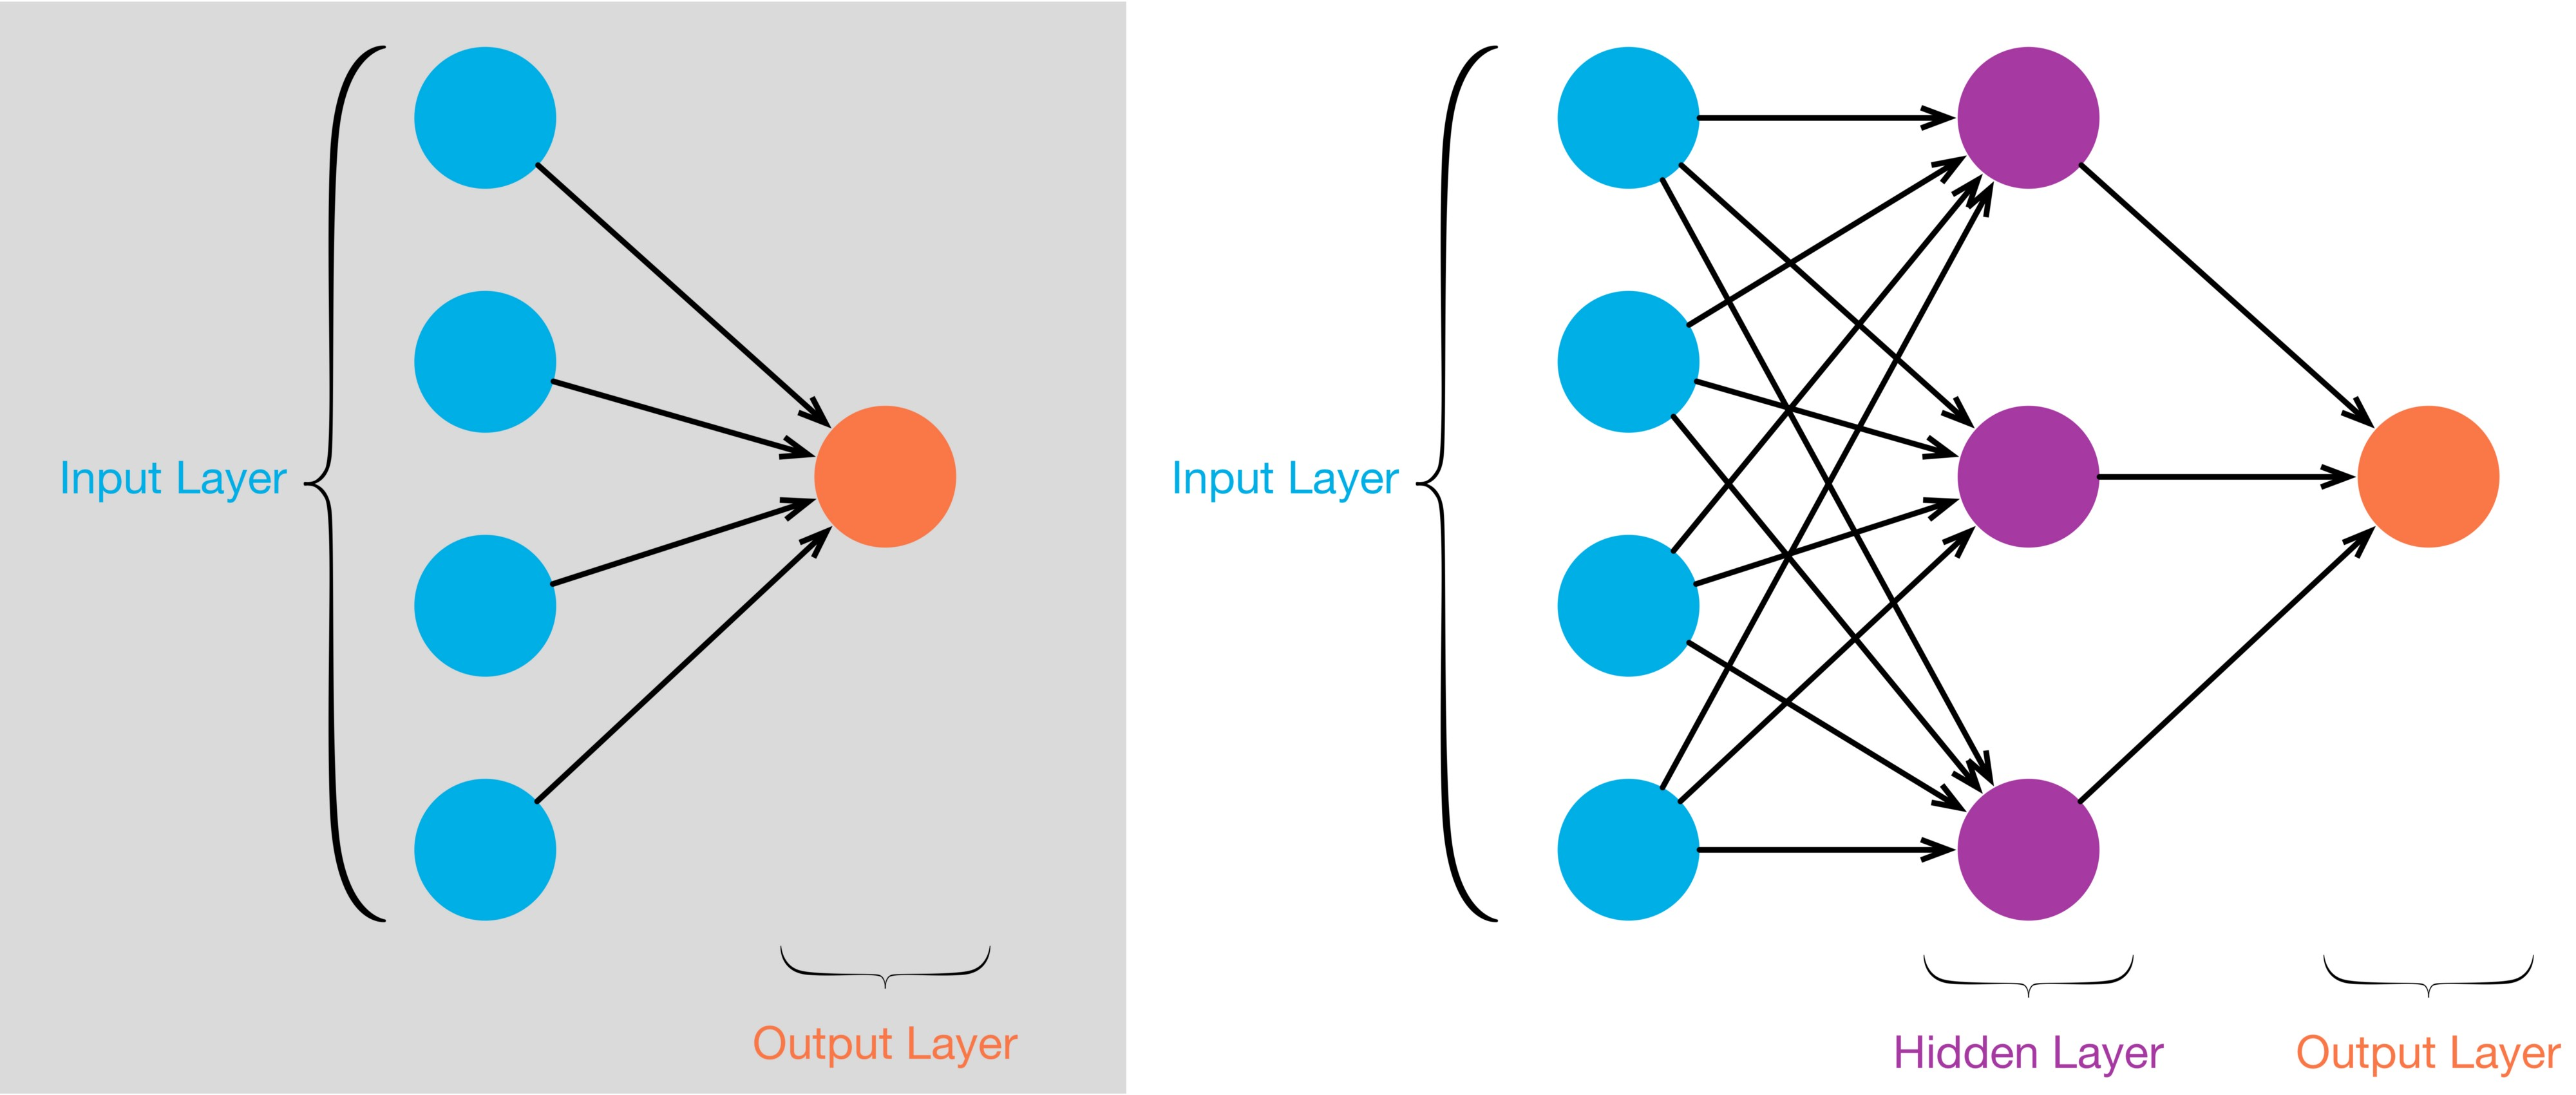
\includegraphics[scale=0.09]{img/nn-layers.jpeg}
\end{center}

The 2-layer neural network has a hidden layer composed of hidden units (the neurons). Note that the input layer is usually ignored when counting the layers. \\

To understand deeply the 1-layer I strongly recommend Andrew Ng's tutorial for more details or this \href{https://towardsdatascience.com/everything-you-need-to-know-about-neural-networks-and-backpropagation-machine-learning-made-easy-e5285bc2be3a}{article} for a wrap up. \\

Let's now go into deeper details on the working on a 2-layer network.

\section{2-layer NN}

There are already an elephantic number of articles and resources on the maths behind neural networks, so I won't go into much details but rather focus on the points that are, in my view, the most important. \\

For the sake of simplicity, we will use a binary classification to build the playground. Thus, the labels belong to ($\{0,1\}$). The cost function is:

$$\mathcal{L}(y, \widehat{y})=-[y\log(\widehat{y})+(1-y)\log(1-\widehat{y})]$$

Where $y$ is the true label and $\hat y$ its estimation (probability). \\

We notice that the loss function decreases when $y \neq \widehat y$, which is expected as we want to penalize wrong classification.

The forward propagation allows to compute the loss functions based on the weights:

\begin{center}
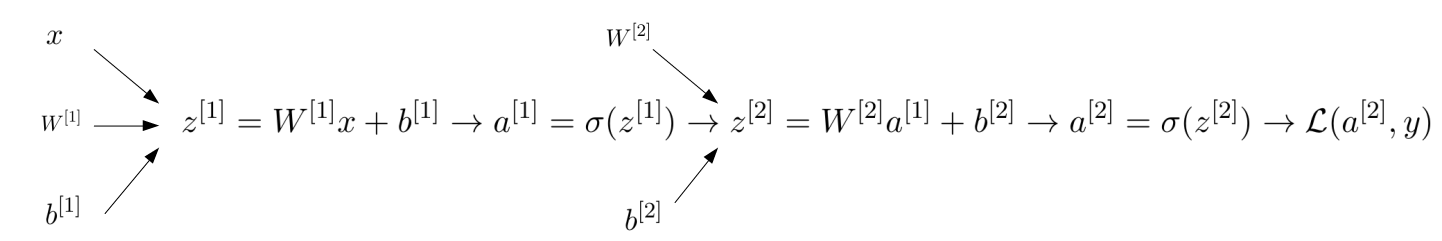
\includegraphics[scale=0.3]{img/NN_2.png}
\end{center}

As we can see here, we use two sets of weights and biases: $W^{[1]}$, $b^{[1]}$, $W^{[2]}$ and $b^{[2]}$. \\

Then, the backward propagation allows to find how to update the weights in order to minimize the loss:

\begin{center}
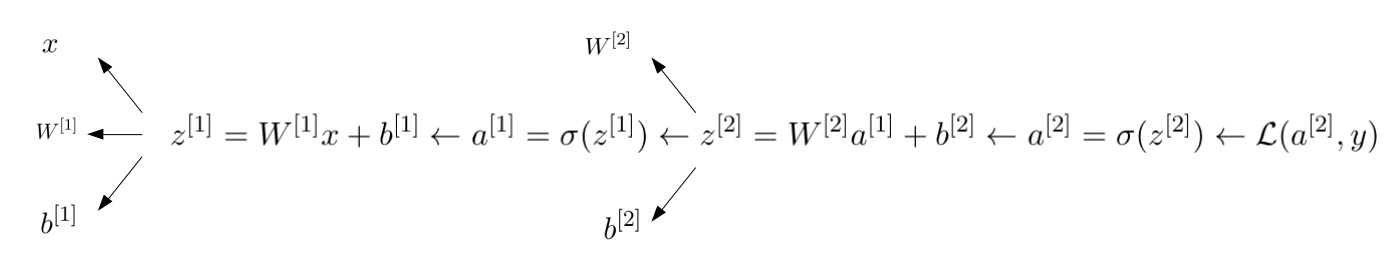
\includegraphics[scale=0.3]{img/NN_2_backward.png}
\end{center}

Starting from the loss' derivative and thanks to the chain rule, we end up with expressions that tell us how to update the weights to minimize the loss.

For the full details on the derivative computation, I wrote down everything on \href{https://savoga.github.io/machinelearning/neural-network/}{my website} (hopefully I didn't do too many mistakes).

\section{Building the app}

The app will allow the user to provide two types of input: \\

- the shape of the data: blobs, circles or moons \\

- the number of hidden units in the neural network \\

Of course, this is just an example of what types of interactions you can have between the user and the neural network. But as explained in the conclusion of the article, you can add much more parameters! \\

The chosen graphical library for the playground is plotly-dash. I am personnaly a big fan of this framework as the \href{https://dash.plotly.com/}{documentation} is quite complete and the \href{https://community.plotly.com/c/dash/16}{community} very active. \\

When developing an app, it is a good practice to separate the modelling part from the graphical part. We will also create a specific module to generate the data. In the end there are 3 python scripts in this app: \\

- app.py: this script creates the server and contains everything about the graphical part (buttons, titles etc.) \\

- model.py: here we implement the neural network itself! \\

- utils.py: in this module we simulate data based on the user's preferences \\

\subsection{app.py}

This module creates the server and handle all graphical components. We specify the location of texts, buttons and the figure. One remark is that we use the same function (also called 'callback functions') for the two buttons. Indeed, it seems plotly-dash doesn't allow to handle different buttons with the same output (= update the graph).

\subsection{model.py}

In this module we build the neural network logic. As mentioned earlier, we want to build it from scratch so that we understand everything what is happening. 

The tricky part here is to be consistent with the dimensions, especially during the derivative computation:

\lstset{language=Python}
\lstset{frame=lines}
\lstset{caption={Backward propagation}}
\lstset{label={lst:code_direct}}
\lstset{basicstyle=\footnotesize}
\begin{lstlisting}

dz2 = a2-y_train
dw2 = (1/n_samples)*np.dot(dz2,a1.T)
db2 = (1/n_samples)*np.sum(dz2)
dz1 = np.multiply(np.dot(self.weights_2.T,dz2),1-np.power(a1,2))
dw1 = (1/n_samples)*np.dot(dz1,X_train.T)
db1 = (1/n_samples)*np.sum(dz1, axis = 1, keepdims = True)

\end{lstlisting}


The full code can be found on my href{https://github.com/savoga/nn-playground-from-scratch/}{Github repo}. \\

\subsection{utils.py}

We will allow the user to choose between three types of data shape: blobs, circles and moons. \\

\begin{center}
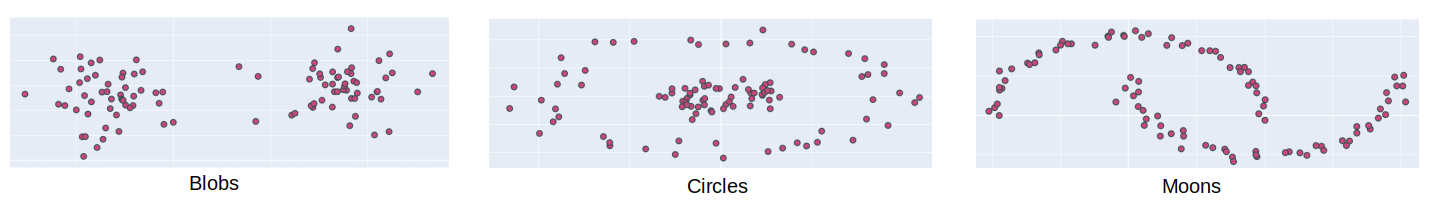
\includegraphics[scale=0.3]{img/data_generation.png}
\end{center}

\section{Deployment}

The deployment is done via \href{https://www.heroku.com/}{Heroku}. The clear steps for deployment are explained \href{https://dash.plotly.com/deployment}{here}. As mentioned in the link, "Heroku is one of the easiest platforms for deploying and managing public Flask applications.".

To sum up, the deployment consists in hosting the code in a Github repo, then deploying through Heroku with this command:

\lstset{language=bash}
\lstset{frame=lines}
\lstset{caption={Deploy the app}}
\lstset{label={lst:code_direct}}
\lstset{basicstyle=\footnotesize}
\begin{lstlisting}

$ git push heroku master

\end{lstlisting}

\vspace{5mm}

\section{Key insights}

When playing with the app we can already draw some interesting insights: \\

- 1 hidden unit gives a linear separation through one line only. This is especially visible when selecting circles. \\

\begin{center}
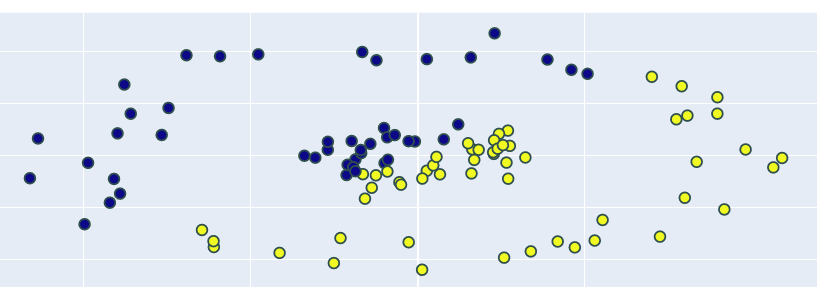
\includegraphics[scale=0.3]{img/1-hu-linear.png}
\end{center}

- 2 hidden unit gives a linear separation through two lines and thus allow a better separation. \\

\begin{center}
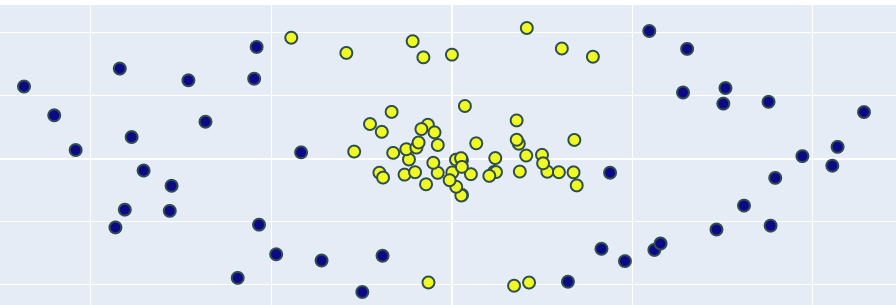
\includegraphics[scale=0.3]{img/2-hu-linear.png}
\end{center}

- 3 hidden units perfectly separates the data when the shapes are not convex (moons).

\begin{center}
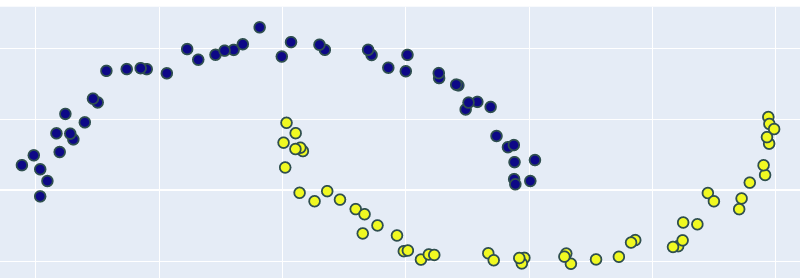
\includegraphics[scale=0.3]{img/3-hu-moons.png}
\end{center}

This illustrates the power of neural networks. We can think of how good they can be when identifying human faces or finger prints!

\section{Extensions}

The extension possibilities are endless! You can think about adding checkboxes/buttons so that the user can choose: \\

- the noise (standard deviation) associated with the data generation

- the number of data points to be generated

- the learning rate to be used during the parameter update

- the number of layers \\

For the last point however, I believe it would require significantly more work, especially if you don't use any neural network library (like tensorflow or pytorch) as we do here. \\

\section{Conclusion}

For the final version of the playground, check out \href{https://nn-playground-app.herokuapp.com/}{this link}. All the code is available on my \href{https://github.com/savoga/nn-playground-from-scratch/}{github repo}. \\

Have fun! \\

PS: This is my first article on Medium, I'd be happy to get your feedback with a clap and/or a comment. \\

\end{document} 
